% !TEX TS-program = XeLaTeX
% !TeX program = xelatex

\documentclass[10pt,a4paper]{article}
\usepackage[a4paper,left=13mm,right=13mm,top=20mm,bottom=15mm]{geometry}

\usepackage{booktabs}
\usepackage{float}
\usepackage[table]{xcolor}
\usepackage{pgfplots}
\usepackage{graphicx}
\usepackage{xurl}
\usepackage{hyperref}
\usepackage{fancyhdr}
\usepackage{abstract}
\usepackage{siunitx}
\usepackage{enumitem}
\usepackage{caption}
\usepackage{multicol}

\usetikzlibrary{arrows.meta,positioning,calc,patterns}

\definecolor{cbase}{RGB}{239,241,245}
\definecolor{ctext}{RGB}{76,69,105}
\definecolor{cflamingo}{RGB}{221,120,120}
\definecolor{cblue}{RGB}{30,102,245}
\definecolor{cgreen}{RGB}{64,160,43}
\definecolor{cred}{RGB}{210,15,57}
\definecolor{cmauve}{RGB}{136,57,239}
\definecolor{cpeach}{RGB}{254,100,11}

\pgfplotsset{compat=1.18}
\pgfplotsset{every axis/.append style={
    tick label style={font=\scriptsize}, label style={font=\small}, title style={font=\small\bfseries},
    grid=both, minor tick num=1,
    major grid style={line width=0.4pt,draw=gray!55}, minor grid style={line width=0.3pt,draw=gray!30}}}

\hypersetup{colorlinks=true, linkcolor=black, filecolor=cblue, urlcolor=cblue, citecolor=cblue}

\setlength{\abovecaptionskip}{3pt}
\setlength{\belowcaptionskip}{0pt}
\captionsetup{font=small,labelfont=bf}
\setlist{nosep,leftmargin=*,itemsep=1pt}
\renewcommand{\abstractnamefont}{\normalfont\large\bfseries}
\setlength{\absleftindent}{0pt}
\setlength{\absrightindent}{0pt}
\setlength{\headheight}{14pt}
\setlength{\parskip}{0pt}
\setlength{\textfloatsep}{6pt plus 2pt minus 2pt}
\setlength{\multicolsep}{4pt plus 1pt minus 1pt}
\renewcommand{\topfraction}{0.92}
\renewcommand{\textfraction}{0.06}
\renewcommand{\floatpagefraction}{0.8}
\setcounter{topnumber}{4}
\setlength{\floatsep}{6pt plus 2pt minus 2pt}
\setlength{\intextsep}{6pt plus 2pt minus 2pt}

\pagestyle{fancy}
\fancyhf{}
\fancyhead[L]{\small Parallel \& Distributed Systems}
\fancyhead[R]{\small Image Denoising and Edge Detection -- OpenMP \& CUDA}
\fancyfoot[C]{\thepage}
\renewcommand{\headrulewidth}{0.4pt}

\begin{document}

\begin{center}
	{\LARGE\bfseries Batch Image Denoising and Edge Detection\\[2pt] with OpenMP and CUDA\par}
	\vspace{0.3cm}
	{\large\textbf{Gerasimou Dimitrios} AEM: 10813 \quad and \quad \textbf{Stavrianidis Giannis} AEM: 11065\\}
	\vspace{0.2cm}
	Department of Electrical and Computer Engineering, Aristotle University of Thessaloniki\\
	050: Parallel and Distributed Systems\\ \vspace{0.2cm}
	Thessaloniki, Greece\\ September 2026
\end{center}

\vspace{0.1cm}
\thispagestyle{empty}

\begin{abstract}
\small
For this assignment, we present a batch tool that denoises grayscale images with \emph{Non-Local Means} (NLM) and extracts their edges
with the \emph{Canny} detector, on multicore CPUs (\textbf{OpenMP}) and on NVIDIA GPUs (\textbf{CUDA}).
The noise level and the filter strength are estimated for every image, and the CPU and the GPU produce identical \textbf{deterministic} output.
The main techniques are integral images for the patch distances, row \textbf{bands} of 16--32 rows drawn from one shared pool
on the CPU, and a shared-memory tile kernel with a register sliding window, a batch pipeline and a two-slot CUDA stream driver on the GPU.
On an Intel i7-11800H and an RTX~3060 Laptop GPU, tested on \num{36669} images of four datasets (two chest X-ray collections with added
Poisson noise, AAPM low-dose CT, and the real noise of 2DeteCT), denoising runs at 1.1\,Mpx/s on one thread, \mbox{7.0--7.3\,Mpx/s} on 16
threads and \mbox{143--149\,Mpx/s} on the GPU: \textbf{20--21$\times$ faster than the CPU and 128--139$\times$ faster than one thread}.
The PSNR rises by 4.5--9.2\,dB on average, and the edge F1 score on 2DeteCT from 0.25 to 0.75.
\end{abstract}

\section{Introduction}
X-ray and CT images are noisy, and the noise breaks the edge detection that often follows. Non-Local Means \cite{buades05,buades11} removes
it by averaging every pixel with all pixels whose surroundings look alike, which preserves structure, but the direct method costs
$(2S{+}1)^2(2P{+}1)^2\approx\num{11025}$ operations per pixel with the usual $21\times21$ search window and $5\times5$ patches: about
$10^{14}$ operations for the \num{8.3} gigapixels of one of our datasets. This work parallelizes the pipeline (read, decode, denoise, detect
edges, encode, write) for batches of images on the CPU and the GPU, and measures its speed and the quality of its output.

\section{Algorithms}
\textbf{Non-Local Means} Every output pixel is the weighted mean of the pixels in its search window. The weight of a candidate falls
exponentially with the squared distance between the two patches, $w=e^{\frac{-\max(d^2 - 2\sigma^2, 0)}{h^2}}$ with $h=k\sigma$ \cite{buades11}, where $d^2$ is the mean squared difference of the two patches.
For a fixed search offset, the squared differences of all pixels form an image, and its \emph{integral image} (summed-area table
\cite{crow84,darbon08}) gives every patch sum with four lookups, which removes the patch size from the cost. Patch sums are exact 32-bit
integers (the integral images wrap around modulo $2^{32}$, which leaves their differences exact), so the result does not depend on the thread count and is the same on the GPU. \textbf{Noise level and strength.} $\sigma$ is
estimated per image as the larger of Immerk{\ae}r's estimate \cite{immerkaer96}, exact for white noise but too low for the correlated
noise of CT reconstructions, and the noise of the flattest $16\times16$ blocks. The strength $k=\frac{h}{\sigma}$ rises from 0.7 (white noise)
to 1.6 (strongly correlated noise) with the ratio of the two estimates. When edge detection follows, it is 0.7 times that for near-white
noise, since the edge score peaks at a milder strength than the PSNR.

\textbf{Canny} \cite{canny86}: Gaussian blur ($\sigma=1.4$), Sobel gradient, non-maximum suppression and hysteresis (thresholds 20 and
50), all in integer arithmetic (fixed-point weights, squared magnitudes), so that both backends agree exactly.

\textbf{Quality} is measured by the PSNR against the ground truth, and by the \emph{edge F1}: the Canny edges of the noisy (or denoised)
image against those of the ground truth, with a tolerance of one pixel.

\section{Parallelization Strategies}
\textbf{Batch pipeline} Images are processed in batches of $B$ (256 by default). The stages run one after the other on a batch, each
parallel over its images. With the GPU, the CPU threads read, decode and prepare batch $k{+}1$ and encode and write batch $k{-}1$
while the GPU works on batch $k$. On the CPU alone it gains nothing, since decoding and encoding already keep all cores busy (the
idle time was 0.3\% of a run). With the GPU it hides all CPU work (Section~\ref{sec:opt}).

\textbf{Bands on the CPU} Every image is cut into horizontal \textbf{bands} of 16--32 rows, about four per thread over the batch,
and the bands of \emph{all} images of the batch, wider images first, form one pool from which the threads draw with
\texttt{schedule(dynamic)}. With fewer images than threads, each image gets a multiple of the thread count of bands, so a single
image keeps every thread busy. This is the only CPU scheduling. Canny uses the same bands.

\begin{itemize}
	\item \textbf{Cache} For one search offset the integral image has one 4-byte entry per pixel: 4\,MB for a 1\,Mpx slice,
	      rebuilt for each of the 441 offsets. For a band of 32 rows of a 1024-pixel-wide image, the integral images of the 4 offsets processed together
	      (0.6\,MB) and the three accumulators per pixel (weight sum, weighted sum, largest weight; 0.4\,MB) take about 1\,MB, which fits
	      the core's L2 cache (1.25\,MB). The scratch of a thread grows with the image width (about 3\,MB for the widest X-rays) but not with its height.
	\item \textbf{Load balance} Our images range from $144\times124$ to $2916\times2863$ pixels. With one image per thread
	      every batch waits for its largest image (97.2\% of the threads busy on the X-ray set). With small equal-cost bands
	      the idle time at the end of a batch is at most one band (99.9\% busy, 15.99 of 16 threads).
	\item \textbf{Independence} A band needs only its own rows of the padded image plus $2P$ margin rows, so there is no
	      synchronization between offsets or threads. The price is the margin: $2P$ of the $\text{band}{+}2P$ difference rows
	      are recomputed. Canny bands recompute the $4+2\cdot$radius blur rows the same way. The thread that finishes the
	      last band of an image runs its hysteresis flood fill at once, while the others continue with other images.
\end{itemize}

\textbf{The GPU kernel} A block of $32\times16$ threads computes a $32\times32$ tile (two pixels per thread). All threads compute
the horizontal patch sums of the four offsets straight from the tile, holding a sliding window of squared differences in registers.
After one barrier each thread slides a vertical window down its two pixels and accumulates the weights, in the same order as the CPU.
The kernel is a C++ template over $P$ (0--10), so the window lives in registers and every division is by a constant. The weights come
from the same function \texttt{nlm\_weight()} as the CPU's table, built from adds, multiplies and explicit \texttt{fmaf}, so the two
results are identical (\texttt{-fmad=false}, \texttt{-ffp-contract=off}).

\textbf{Streams} Images alternate between two \emph{slots}, each with its own CUDA stream, device buffers and pinned host memory.
While an image's kernels run, the next image is uploaded and the previous one downloaded. \textbf{Canny on the GPU} uses one thread
per pixel for blur, gradient and suppression. \textbf{Hysteresis} is a connectivity problem, like the connected components of the
earlier assignments: each $32\times32$ tile spreads edges in shared memory until nothing changes, and the host relaunches until no
tile changes. Only tiles whose neighbours changed a border pixel are \emph{active} in the next launch, and with \texttt{-d -e} the
denoised image stays on the GPU.

\section{Performance Optimizations}\label{sec:opt}
Table~\ref{tab:opt} lists the techniques in order of the measured effect, each measured on the code immediately before it was applied.
The bases differ, so the factors are not multiplied. The GPU steps were guided by profiling (Nsight Compute): idle lanes (42\% lane
use in the difference phase), then shared-memory traffic (MIO throttle, 43\% of the stalls) and bank conflicts (45\% of the
shared-memory cycles were wasted), and on noisy images the weight-table gathers, which missed the L1 cache (12.9\% hits against 98.8\%
on clean images).

\begin{table}[H]
	\centering\footnotesize
	\rowcolors{2}{gray!22}{white}
	\begin{tabular}{p{10.8cm}p{5.3cm}}
		\toprule
		\textbf{Technique} & \textbf{Effect}\\
		\midrule
		NLM on the GPU (all techniques below) & 20--21$\times$ over 16 threads, 128--139$\times$ over 1 thread\\
		Integral images for the patch sums, with a weight table (CPU) & 5.6$\times$\\
		GPU kernel restructuring v1$\to$v4: no integer division, 32-row tiles with 2 pixels per thread, dense element mapping, register window, 4 offsets per barrier, template over $P$ & 3.2$\times$\\
		Bands and fast interior path for Canny (CPU) & 3.0$\times$, threads busy 9.7 $\to$ 15.6\\
		Table-free weights on the GPU (no table gathers) & 1.49$\times$\\
		Batch pipeline with the GPU (batches of 16 instead of one batch) & 1.24$\times$\\
		Offset blocking on the CPU: 4 offsets per pass, independent running sums & 1.14$\times$ at 16 threads, 1.17--1.48$\times$ at 1\\
		Chunked rejection: branch-free sums, 16 pixels skipped at once & 1.10--1.18$\times$\\
		Active tiles in the GPU hysteresis & hysteresis $-$28\%\\
		Explicit \texttt{fmaf} in the weight polynomial; conflict-free tile pitch with one 16-byte store & 1.06$\times$; 1.04$\times$\\
		Band pool with dynamic scheduling (load balance) & threads busy 97.2\% $\to$ 99.9\% ($\approx$3\%)\\
		Pinned memory with two streams & downloads 3.6$\times$ faster, $-$5\% (edges only)\\
		\bottomrule
	\end{tabular}
	\caption{Optimization techniques ranked by measured effect. Overall, the CPU version became 10.7$\times$ faster than the first direct implementation.}
	\label{tab:opt}
\end{table}

\textbf{Tried and rejected} \texttt{-march=native} gave nothing. The loops are limited by the integral image's dependency
chain and by data-dependent branches, not by vector width. Skipping weights below $10^{-3}$ (as OpenCV does) was 18--24\%
\emph{slower} on noisy images, since the accept/reject branch becomes unpredictable, and changed the output. Preselecting
candidates by local statistics \cite{mahmoudi05,coupe08} saves little, as a rejection already costs only four lookups.
Symmetric weights would break the bit-exact match with the reference.

\section{Experimental Setup}
\textbf{System:} Intel Core i7-11800H (8 cores, 16 threads, 1.25\,MB L2 per core), 15.3\,GiB RAM, NVIDIA GeForce RTX~3060
Laptop GPU (compute capability 8.6, 30 multiprocessors, 5.7\,GiB), Arch Linux, CUDA 13.4, \texttt{gcc -O3 -fopenmp},
\texttt{nvcc -O3}, performance governor, threads bound with \texttt{OMP\_PROC\_BIND=close OMP\_PLACES=cores}.
\textbf{Speed} is measured on a random sample of 500 images of each dataset: a thread sweep on the CPU (batch of 64) and
a batch sweep (4--256) on the CPU and the GPU, for denoising and for edge detection, with one warmup and three timed trials
(median). The pipeline time covers reading, decoding and filtering (no output). \textbf{Quality} is measured on every image,
and the complete datasets are also timed end to end (batches of 16, output written, one trial). All runs use the default options. The datasets (\num{36669} images) are:

\begin{itemize}
	\item \textbf{Chest X-ray (pneumonia)}: the \num{5856} pediatric radiographs of the Kaggle pneumonia set
	      \cite{kermany18}. Poisson noise (dose drawn per image from 10--50\%, seed 0) is added to the originals, which are the ground truth.
	\item \textbf{Chest X-ray (mixed)}: \num{25553} radiographs of mixed origin (\num{10641} tuberculosis,
	      \num{9088} normal, \num{5824} pneumonia cases), $144\times124$ to $2916\times2863$ pixels (Kaggle
	      \cite{kagglecxr}). Poisson noise is added as for the previous set.
	\item \textbf{AAPM Low-Dose CT}: \num{4260} slices of $512\times512$ \cite{mccollough17}, from a community \texttt{.npy} mirror. The quarter-dose
	      slice is the input, the full-dose slice the truth.
	\item \textbf{2DeteCT}: \num{1000} slices of $1024\times1024$ \cite{kiss23}. The mode-1 (low dose)
	      reconstruction is the input and the mode-2 (high fidelity) reconstruction the truth. The noise of
	      both is real or simulated on the projections, and spatially correlated.
\end{itemize}
The CT slices are mapped to 8 bits with one window per dataset, from 0 to the 99.5th percentile of the reference images, so the PSNR values are relative to that window.

\section{Results}
\subsection{Speed}
Table~\ref{tab:speed} and Figure~\ref{fig:speed} summarize the 500-image sweeps. \textbf{Denoising costs the same per
pixel on every dataset}, whatever the noise level, strength or image size: 1.1\,Mpx/s on one thread, 7.0--7.3\,Mpx/s
on 16 threads, 143--149\,Mpx/s on the GPU. The CPU scales 6.4--6.5$\times$ on 16 threads, and already 6.3--6.5$\times$
on 8 (80\% efficiency). The machine has 8 physical cores, and hyperthreading adds only 0.1--2.7\% to denoising, but
14--22\% to the edge detection. The GPU is \textbf{20--21$\times$ faster than the best CPU run} for denoising and
2.9--5.7$\times$ for edges, where decoding the PNG files takes about as long as the filter and limits the gain, most
on the smallest images (AAPM). On the GPU, batches of 4--16 images are fastest for denoising and 64 for edges. A batch
of 256 is 8--13\% slower and needs 3--6$\times$ the memory of a batch of 16, while the CPU time hardly depends on the
batch size above 16.

\textbf{Batch size} Figure~\ref{fig:batch}(a) shows the time of each configuration relative to its best batch size, averaged over the
four datasets. Small batches hurt most where the work per image is smallest: GPU edge detection is 2.9$\times$ slower with 4 images per batch
than with 64, CPU edge detection 1.6$\times$, GPU denoising 17\%, while CPU denoising stays within 8\%. Each batch pays a fixed cost
(stage barriers, filling and draining the pipeline) that fewer images share. Large batches do not make it faster: from 16 to 256 images
the memory of the GPU run grows 3--6$\times$ (Figure~\ref{fig:batch}(b)) and that of the CPU run 3--9$\times$, and the GPU denoising becomes 10\% slower, most
likely because the pipeline overlaps only the batches after the first, and 500 images make two batches of 256. A batch of 16--64 is the best
compromise.

\begin{table}[H]
	\centering\footnotesize
	\rowcolors{2}{gray!22}{white}
	\setlength{\tabcolsep}{5pt}
	\begin{tabular}{lrrrrrrrrrrr}
		\toprule
		& & \multicolumn{3}{c}{\textbf{Denoising time (s)}} & \multicolumn{3}{c}{\textbf{Speedup}} & \multicolumn{3}{c}{\textbf{Edge detection time (s)}} & \textbf{Speedup}\\
		\cmidrule(lr){3-5}\cmidrule(lr){6-8}\cmidrule(lr){9-11}
		\textbf{Dataset} & \textbf{Mpx} & 1 thr. & 16 thr. & GPU & 16/1 thr. & GPU/16 & GPU/1 & 1 thr. & 16 thr. & GPU & GPU/16\\
		\midrule
		Chest X-ray (pneumonia) & 710 & 636.8 & 100.2 & 4.97 & 6.4$\times$ & 20.1$\times$ & 128$\times$ & 21.05 & 2.68 & 0.596 & 4.5$\times$ \\
		Chest X-ray (mixed) & 341 & 306.3 & 47.6 & 2.36 & 6.4$\times$ & 20.2$\times$ & 130$\times$ & 10.23 & 1.30 & 0.332 & 3.9$\times$ \\
		AAPM Low-Dose CT & 131 & 116.1 & 17.9 & 0.88 & 6.5$\times$ & 20.3$\times$ & 132$\times$ & 4.21 & 0.49 & 0.172 & 2.9$\times$ \\
		2DeteCT & 524 & 490.2 & 75.0 & 3.52 & 6.5$\times$ & 21.3$\times$ & 139$\times$ & 18.58 & 2.27 & 0.400 & 5.7$\times$ \\
		\bottomrule
	\end{tabular}
	\caption{Speed on 500-image samples (best batch size of each run, median of 3 trials).}
	\label{tab:speed}
\end{table}

\begin{figure}[H]
	\centering
	\begin{minipage}[t]{0.345\linewidth}
		\centering
		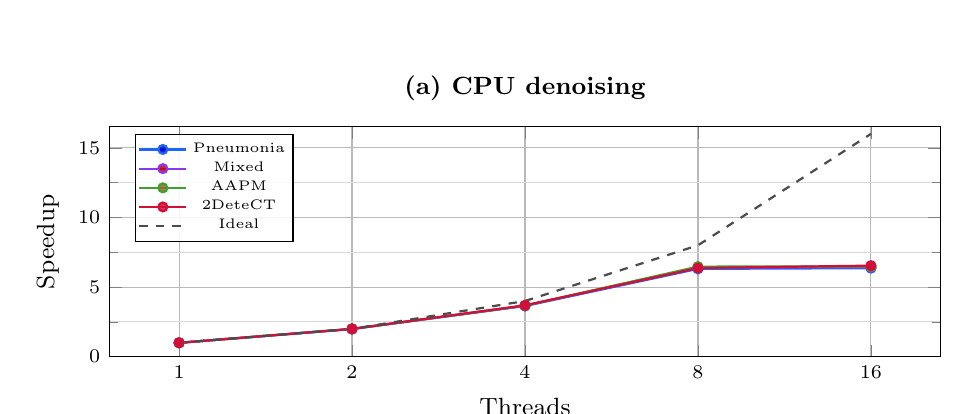
\begin{tikzpicture}
			\begin{axis}[width=\linewidth,height=4.5cm,xmode=log,log basis x=2,xtick={1,2,4,8,16},xticklabels={1,2,4,8,16},ymin=0,ymax=16.5,
			  xlabel={Threads},ylabel={Speedup},title={(a) CPU denoising},legend style={at={(0.03,0.97)},anchor=north west,font=\tiny,inner sep=1pt,row sep=-2pt,fill=white,fill opacity=0.85,text opacity=1}]
				\addplot+[color=cblue,mark=*,mark size=1.6pt,thick] coordinates {(1,1.00) (2,1.99) (4,3.64) (8,6.31) (16,6.36)};
				\addplot+[color=cmauve,mark=*,mark size=1.6pt,thick] coordinates {(1,1.00) (2,1.99) (4,3.67) (8,6.39) (16,6.43)};
				\addplot+[color=cgreen,mark=*,mark size=1.6pt,thick] coordinates {(1,1.00) (2,2.00) (4,3.67) (8,6.47) (16,6.48)};
				\addplot+[color=cred,mark=*,mark size=1.6pt,thick] coordinates {(1,1.00) (2,2.00) (4,3.69) (8,6.37) (16,6.54)};
				\addplot[dashed,black!70,thick,mark=none] coordinates {(1,1) (2,2) (4,4) (8,8) (16,16)};
				\legend{Pneumonia,Mixed,AAPM,2DeteCT,Ideal}
			\end{axis}
		\end{tikzpicture}
	\end{minipage}\hfill
	\begin{minipage}[t]{0.305\linewidth}
		\centering
		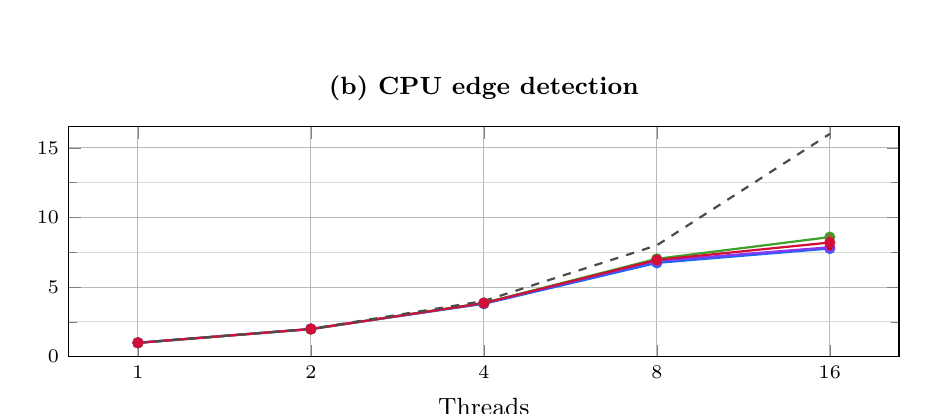
\begin{tikzpicture}
			\begin{axis}[width=\linewidth,height=4.5cm,xmode=log,log basis x=2,xtick={1,2,4,8,16},xticklabels={1,2,4,8,16},ymin=0,ymax=16.5,
			  xlabel={Threads},title={(b) CPU edge detection}]
				\addplot+[color=cblue,mark=*,mark size=1.6pt,thick] coordinates {(1,1.00) (2,1.99) (4,3.80) (8,6.74) (16,7.77)};
				\addplot+[color=cmauve,mark=*,mark size=1.6pt,thick] coordinates {(1,1.00) (2,1.99) (4,3.85) (8,6.88) (16,7.86)};
				\addplot+[color=cgreen,mark=*,mark size=1.6pt,thick] coordinates {(1,1.00) (2,1.98) (4,3.86) (8,7.03) (16,8.59)};
				\addplot+[color=cred,mark=*,mark size=1.6pt,thick] coordinates {(1,1.00) (2,1.99) (4,3.85) (8,6.95) (16,8.20)};
				\addplot[dashed,black!70,thick,mark=none] coordinates {(1,1) (2,2) (4,4) (8,8) (16,16)};
			\end{axis}
		\end{tikzpicture}
	\end{minipage}\hfill
	\begin{minipage}[t]{0.315\linewidth}
		\centering
		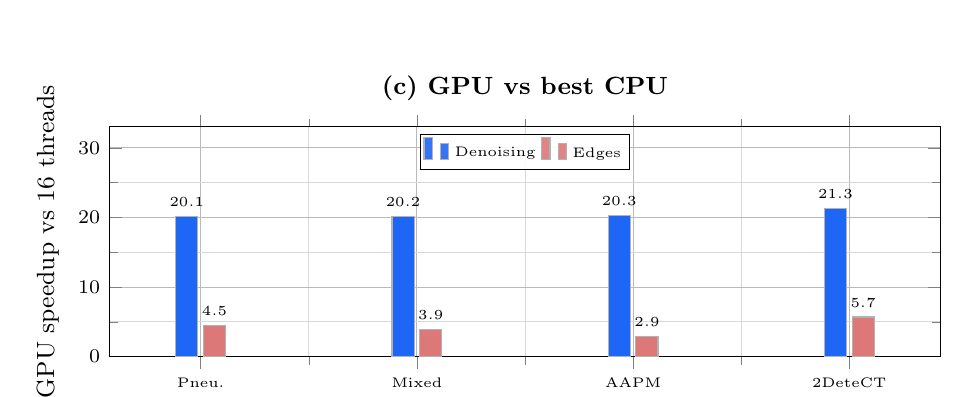
\begin{tikzpicture}
			\begin{axis}[ybar,bar width=8pt,width=\linewidth,height=4.5cm,ymin=0,ymax=33,enlarge x limits=0.14,symbolic x coords={Pneu.,Mixed,AAPM,2DeteCT},xtick=data,x tick label style={font=\tiny},
			  ylabel={GPU speedup vs 16 threads},title={(c) GPU vs best CPU},nodes near coords,nodes near coords style={font=\tiny,text=black},
			  legend style={at={(0.5,0.97)},anchor=north,font=\tiny,legend columns=2,inner sep=1pt,fill=white,fill opacity=0.9,text opacity=1}]
				\addplot+[fill=cblue,draw=black!30] coordinates {(Pneu.,20.1) (Mixed,20.2) (AAPM,20.3) (2DeteCT,21.3)};
				\addplot+[fill=cflamingo,draw=black!30] coordinates {(Pneu.,4.5) (Mixed,3.9) (AAPM,2.9) (2DeteCT,5.7)};
				\legend{Denoising,Edges}
			\end{axis}
		\end{tikzpicture}
	\end{minipage}
	\caption{Speedup of the CPU thread sweeps (a, b) and of the GPU over the best CPU run (c), for the four datasets.}
	\label{fig:speed}
\end{figure}

\begin{figure}[H]
	\centering
	\begin{minipage}[t]{0.49\linewidth}
		\centering
		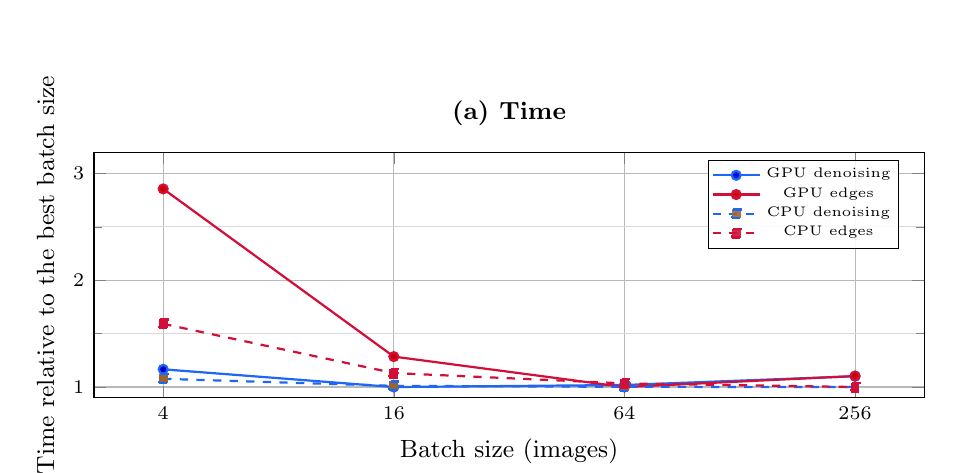
\begin{tikzpicture}
			\begin{axis}[width=\linewidth,height=4.7cm,xmode=log,log basis x=2,xtick={4,16,64,256},xticklabels={4,16,64,256},ymin=0.9,ymax=3.2,
			  xlabel={Batch size (images)},ylabel={Time relative to the best batch size},title={(a) Time},
			  legend style={at={(0.97,0.97)},anchor=north east,font=\tiny,inner sep=1pt,row sep=-2pt,fill=white,fill opacity=0.9,text opacity=1}]
				\addplot+[color=cblue,mark=*,mark size=1.6pt,thick] coordinates {(4,1.166) (16,1.000) (64,1.019) (256,1.101)};
				\addplot+[color=cred,mark=*,mark size=1.6pt,thick] coordinates {(4,2.856) (16,1.285) (64,1.000) (256,1.103)};
				\addplot+[color=cblue,mark=square*,mark size=1.6pt,thick,dashed] coordinates {(4,1.077) (16,1.011) (64,1.002) (256,1.000)};
				\addplot+[color=cred,mark=square*,mark size=1.6pt,thick,dashed] coordinates {(4,1.592) (16,1.131) (64,1.034) (256,1.000)};
				\legend{GPU denoising,GPU edges,CPU denoising,CPU edges}
			\end{axis}
		\end{tikzpicture}
	\end{minipage}\hfill
	\begin{minipage}[t]{0.49\linewidth}
		\centering
		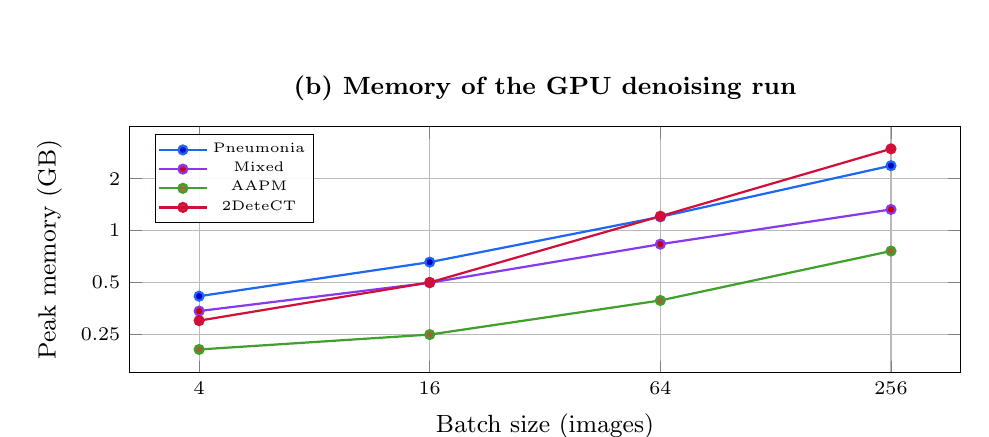
\begin{tikzpicture}
			\begin{axis}[width=\linewidth,height=4.7cm,xmode=log,log basis x=2,xtick={4,16,64,256},xticklabels={4,16,64,256},ymode=log,ymin=0.15,ymax=4,
			  log ticks with fixed point,ytick={0.25,0.5,1,2},yticklabels={0.25,0.5,1,2},
			  xlabel={Batch size (images)},ylabel={Peak memory (GB)},title={(b) Memory of the GPU denoising run},
			  legend style={at={(0.03,0.97)},anchor=north west,font=\tiny,inner sep=1pt,row sep=-2pt,fill=white,fill opacity=0.9,text opacity=1}]
				\addplot+[color=cblue,mark=*,mark size=1.6pt,thick] coordinates {(4,0.416) (16,0.656) (64,1.202) (256,2.382)};
				\addplot+[color=cmauve,mark=*,mark size=1.6pt,thick] coordinates {(4,0.341) (16,0.498) (64,0.834) (256,1.327)};
				\addplot+[color=cgreen,mark=*,mark size=1.6pt,thick] coordinates {(4,0.204) (16,0.249) (64,0.393) (256,0.761)};
				\addplot+[color=cred,mark=*,mark size=1.6pt,thick] coordinates {(4,0.300) (16,0.500) (64,1.212) (256,2.984)};
				\legend{Pneumonia,Mixed,AAPM,2DeteCT}
			\end{axis}
		\end{tikzpicture}
	\end{minipage}
	\caption{Effect of the batch size (500-image sweeps). (a) Time relative to the best batch size of each configuration, mean of the four datasets, the CPU with 16 threads. (b) Peak resident memory of the GPU denoising run, per dataset.}
	\label{fig:batch}
\end{figure}

\subsection{Complete Datasets}
Table~\ref{tab:full} gives the end-to-end times of the runs on every image of each dataset: read, decode, filter, encode and write the
result, with 16 threads, batches of 16 and one trial. The GPU is 20--22$\times$ faster than the CPU here as well (16.6--20.5$\times$ when edges follow),
although every result image is encoded and written: the batch pipeline hides this CPU-side work behind the kernels, and the whole run reaches
142--150\,Mpx/s, as in the 500-image sweeps. The CPU needs 20 minutes for the pneumonia set and 44 minutes for the mixed set, the GPU 58 and 130 seconds.
Edge detection after the denoising adds 1--3\% on the CPU and 8--10\% on the GPU, and 21\% on the small AAPM slices, where decoding dominates.

\begin{table}[H]
	\centering\footnotesize
	\rowcolors{2}{gray!22}{white}
	\setlength{\tabcolsep}{5pt}
	\begin{tabular}{lrrrrrrrrrr}
		\toprule
		& & & \multicolumn{4}{c}{\textbf{Denoising time (s)}} & \multicolumn{4}{c}{\textbf{Denoising \& Canny time (s)}}\\
		\cmidrule(lr){4-7}\cmidrule(lr){8-11}
		\textbf{Dataset} & \textbf{Images} & \textbf{Mpx} & CPU & GPU & Speedup & GPU Mpx/s & CPU & GPU & Speedup & GPU Mpx/s\\
		\midrule
		Chest X-ray (pneumonia) & 5\,856 & 8\,309 & 1\,186.1 & 57.7 & 20.5$\times$ & 144 & 1\,210.0 & 62.4 & 19.4$\times$ & 133 \\
		Chest X-ray (mixed) & 25\,553 & 18\,486 & 2\,635.2 & 130.0 & 20.3$\times$ & 142 & 2\,691.8 & 143.1 & 18.8$\times$ & 129 \\
		AAPM Low-Dose CT & 4\,260 & 1\,117 & 153.2 & 7.7 & 20.0$\times$ & 145 & 154.7 & 9.3 & 16.6$\times$ & 120 \\
		2DeteCT & 1\,000 & 1\,049 & 151.9 & 7.0 & 21.7$\times$ & 150 & 156.0 & 7.6 & 20.5$\times$ & 138 \\
		\bottomrule
	\end{tabular}
	\caption{End-to-end times on the complete datasets (16 threads, batches of 16, output written, one trial).}
	\label{tab:full}
\end{table}


\subsection{Quality}
Table~\ref{tab:quality} gives the quality on every image of each dataset. The noise added to the chest X-rays is estimated
3--4\% low (10.4 against 10.9, and 10.7 against 11.0 gray levels). Denoising raises the PSNR by 4.5--9.2\,dB on average,
and only \mbox{4 of the \num{36669}} images get worse, by at most 1.6\,dB (all tuberculosis radiographs, which already have
the most reliable noisy edges). The edge F1 rises on every dataset, most where the noisy edges are useless, from 0.25 to
0.75 on 2DeteCT, where every one of the \num{1000} slices improves (Figure~\ref{fig:images}). Where the noisy image is
already reliable, denoising can lower the score. In the cleanest quarter of the AAPM slices the F1 changes by $-0.014$,
and in the cleanest quarter of the mixed chest X-rays 35\% of the images end with a lower edge score than the noisy input.
This is the price of a strength that favours the PSNR. The worst AAPM slice (18.2\,dB) gains only 0.2\,dB. Structured
artifacts are not noise and a denoiser cannot repair them. The 500-image samples agree with the full sets to within
0.14\,dB and 0.004 F1.

\begin{table}[H]
	\centering\footnotesize
	\rowcolors{2}{gray!22}{white}
	\setlength{\tabcolsep}{5pt}
	\begin{tabular}{lrrrrrrrrr}
		\toprule
		& & \textbf{Noise $\sigma$} & \multicolumn{3}{c}{\textbf{PSNR (dB)}} & \multicolumn{3}{c}{\textbf{Edge F1}} & \textbf{F1 lower}\\
		\cmidrule(lr){4-6}\cmidrule(lr){7-9}
		\textbf{Dataset} & \textbf{Images} & added / est. & noisy & denoised & gain & noisy & denoised & gain & than noisy\\
		\midrule
		Chest X-ray (pneumonia) & 5\,856 & 10.9 / 10.4 & 27.63 & 36.87 & +9.24 & 0.691 & 0.800 & +0.110 & 6\% \\
		Chest X-ray (mixed) & 25\,553 & 11.0 / 10.7 & 27.51 & 36.24 & +8.74 & 0.738 & 0.798 & +0.061 & 22\% \\
		AAPM Low-Dose CT & 4\,260 & -- / 12.3 & 26.08 & 30.57 & +4.48 & 0.821 & 0.852 & +0.031 & 32\% \\
		2DeteCT & 1\,000 & -- / 18.6 & 22.77 & 28.46 & +5.69 & 0.249 & 0.749 & +0.500 & 0\% \\
		\bottomrule
	\end{tabular}
	\caption{Quality on all images of each dataset (means). $\sigma$ in gray levels. The last column is the share of images whose edge F1 is lower after denoising.}
	\label{tab:quality}
\end{table}

\begin{figure}[H]
	\centering
	\setlength{\tabcolsep}{2pt}
	\newcommand{\pw}{3.7cm}
	\begin{tabular}{ccc}
		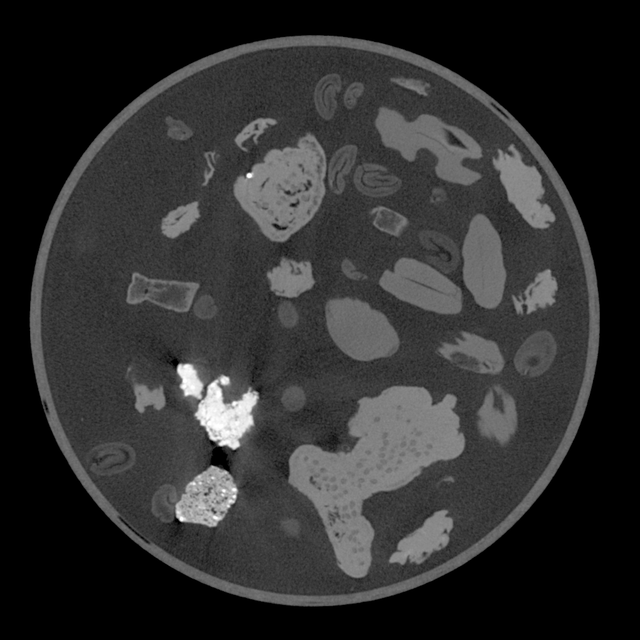
\includegraphics[width=\pw]{figures/p_ref.png} & 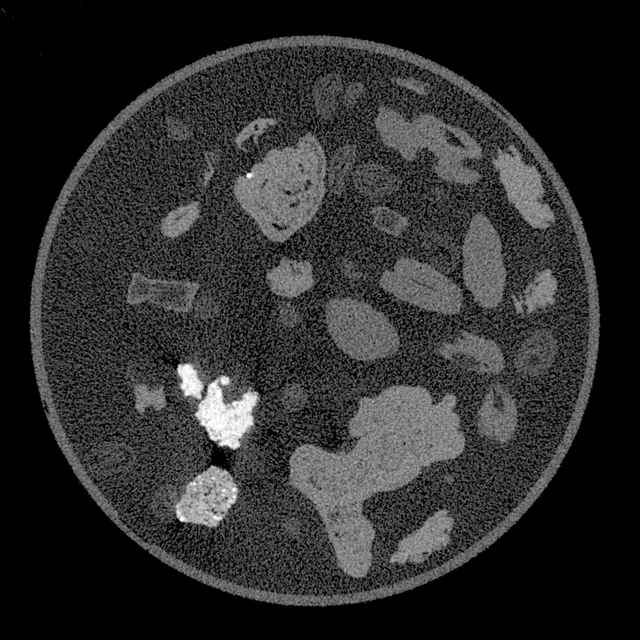
\includegraphics[width=\pw]{figures/p_noisy.png} & 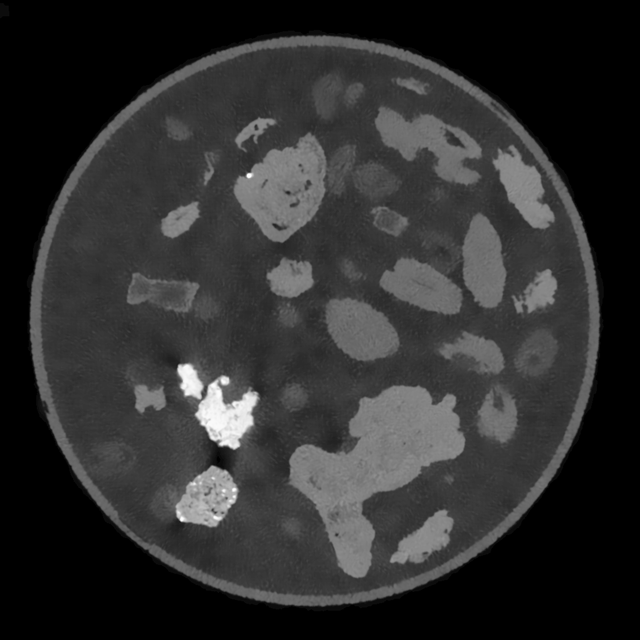
\includegraphics[width=\pw]{figures/p_den.png}\\[-1pt]
		{\footnotesize (a) reference (mode 2)} & {\footnotesize (b) noisy (mode 1)} & {\footnotesize (c) denoised}\\[2pt]
		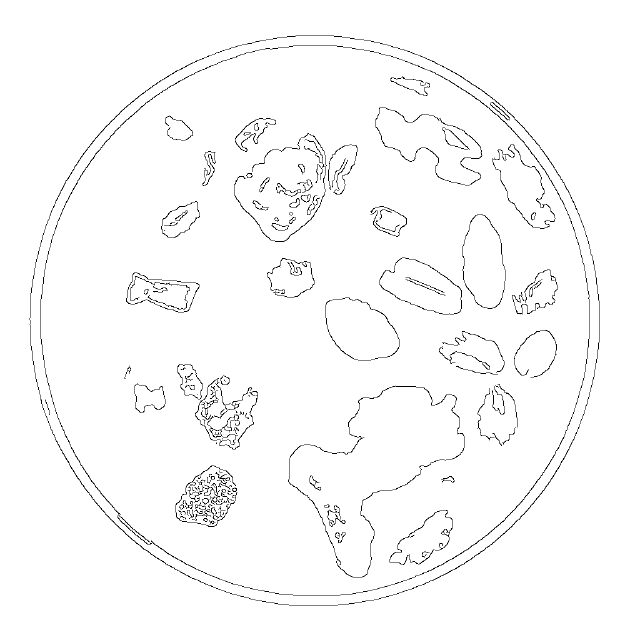
\includegraphics[width=\pw]{figures/p_eref.png} & 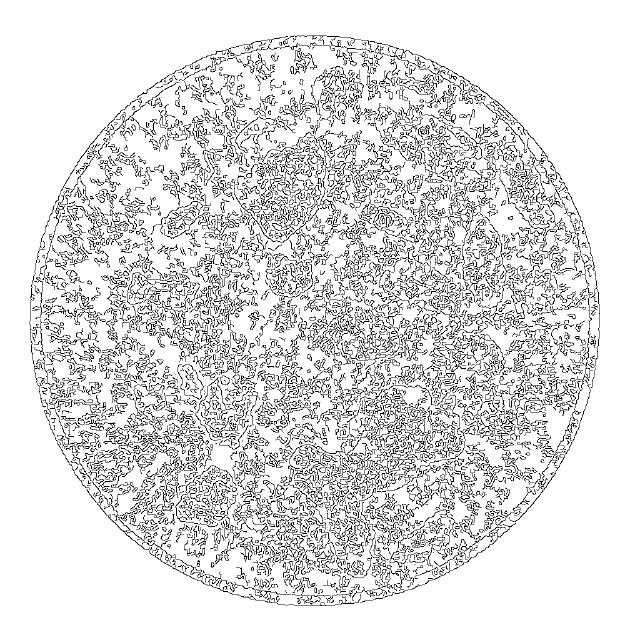
\includegraphics[width=\pw]{figures/p_enoisy.png} & 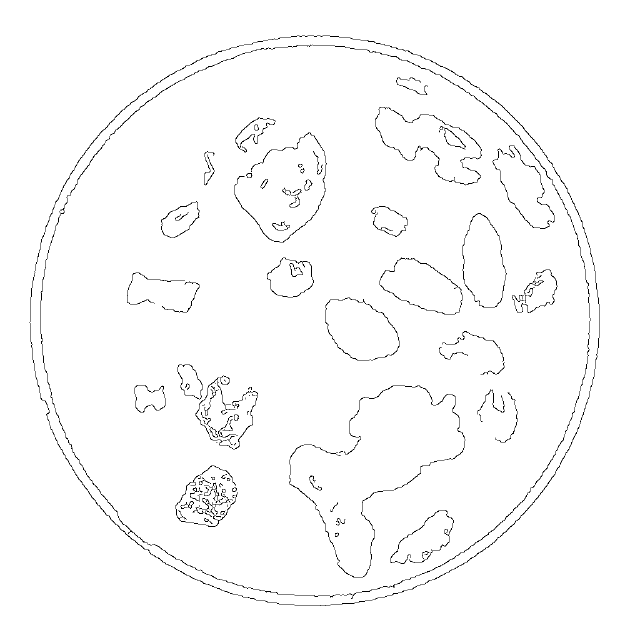
\includegraphics[width=\pw]{figures/p_eden.png}\\[-1pt]
		{\footnotesize (d) edges of (a)} & {\footnotesize (e) edges of (b)} & {\footnotesize (f) edges of (c)}\\
	\end{tabular}
	\caption{One 2DeteCT slice: PSNR 27.9 $\to$ 36.6\,dB, edge F1 0.27 $\to$ 0.87. The Canny edges of the noisy slice (e) are dominated by noise, those of the denoised slice (f) follow the reference (d). Gray images shown with a display gamma of 0.55, edge maps inverted (dark edges).}
\label{fig:images}
\end{figure}

\section{Analysis and Discussion}
\begin{itemize}
	\item \textbf{The GPU suits NLM}: heavy, regular, independent work per pixel. The whole pipeline reaches $\approx$15\,ps
	      per pixel and search offset (the first kernel: 52\,ps), which is 143--149\,Mpx/s. \textbf{Edge detection is the
	      opposite}: cheap per pixel, with decoding and hysteresis (an irregular connectivity problem) dominating, hence
	      only 2.9--5.7$\times$. The copies that are 2\% of the NLM GPU time were 27--42\% of the Canny GPU time before the streams.
	\item \textbf{Efficiency is bounded by the hardware}: 80\% on 8 cores and 40\% on 16 threads. NLM already keeps each core
	      busy, so hyperthreading adds nothing, unlike the memory-bound edge detection (14--22\%).
	\item \textbf{Exactness} made every step testable: the CPU and the GPU agree bit for bit, so each optimization was checked for identical output.
	      An independent float64 NumPy implementation of the same algorithm matches to within one gray level, apart from rare outlier
	      pixels whose candidates all have weights below $e^{-30}$, which the code skips.
\end{itemize}

\section{Conclusions}
\texttt{imgfilter} denoises and edge-detects batches of images on the CPU and the GPU with identical results, and needs no tuning.
Bands of 16--32 rows drawn from one pool make the CPU version scale as far as the eight cores allow (6.4--6.5$\times$).
A profile-driven tile kernel and a two-slot stream pipeline make the GPU \textbf{20--21$\times$ faster than the 16-thread CPU} for
denoising (128--139$\times$ over one thread). The automatic noise estimate and strength raise the PSNR by 4.5--9.2\,dB and the edge
F1 on real CT noise from 0.25 to 0.75.

\textbf{Future work:} Decode PNG on the GPU (it limits the edge speedup). Fuse the Canny kernels and propagate whole rows per
hysteresis iteration. Choose the strength per image for the edge score, since the cleanest slices lose a little. Symmetric weights
with a tolerance based reference. Multi-GPU batches.

\textbf{Code Availability:} Source code, benchmark scripts and the benchmark results (\texttt{docs/performance.md}) are available at:
\url{https://github.com/dimgerasimou/pds-hw4-img-processing}.

\begin{multicols}{2}
\begin{thebibliography}{99}\footnotesize\setlength{\itemsep}{0pt}\setlength{\parskip}{0pt}
\bibitem{buades05} A. Buades, B. Coll, J.-M. Morel, A non-local algorithm for image denoising, \emph{CVPR}, 2005.
\bibitem{buades11} A. Buades, B. Coll, J.-M. Morel, Non-local means denoising, \emph{Image Processing On Line} 1, 2011.
\bibitem{canny86} J. Canny, A computational approach to edge detection, \emph{IEEE TPAMI} 8(6), 1986.
\bibitem{immerkaer96} J. Immerk{\ae}r, Fast noise variance estimation, \emph{Computer Vision and Image Understanding} 64(2), 1996.
\bibitem{crow84} F. C. Crow, Summed-area tables for texture mapping, \emph{SIGGRAPH}, 1984.
\bibitem{darbon08} J. Darbon et al., Fast nonlocal filtering applied to electron cryomicroscopy, \emph{IEEE ISBI}, 2008.
\bibitem{mahmoudi05} M. Mahmoudi, G. Sapiro, Fast image and video denoising via nonlocal means of similar neighborhoods, \emph{IEEE Signal Processing Letters} 12(12), 2005.
\bibitem{coupe08} P. Coup\'e et al., An optimized blockwise nonlocal means denoising filter for 3-D MR images, \emph{IEEE TMI} 27(4), 2008.
\bibitem{kermany18} D. S. Kermany et al., Identifying medical diagnoses and treatable diseases by image-based deep learning, \emph{Cell} 172(5), 2018.
\bibitem{kagglecxr} Kaggle dataset \href{https://www.kaggle.com/datasets/muhammadrehan00/chest-xray-dataset}{\texttt{muhammadrehan00/chest-xray-dataset}}.
\bibitem{mccollough17} C. H. McCollough et al., Low-dose CT for the detection and classification of metastatic liver lesions: results of the 2016 Low Dose CT Grand Challenge, \emph{Medical Physics} 44(10), 2017.
\bibitem{kiss23} M. B. Kiss et al., 2DeteCT -- a large 2D expandable, trainable, experimental computed tomography dataset for machine learning, \emph{Scientific Data} 10, 2023.
\end{thebibliography}
\end{multicols}

\end{document}
